\documentclass{article}
\usepackage{tikz}
\usetikzlibrary{positioning, shapes, fit, math}

\begin{document}

\begin{figure}[h]
    \centering
    \resizebox{\textwidth}{!}{
    \centering
    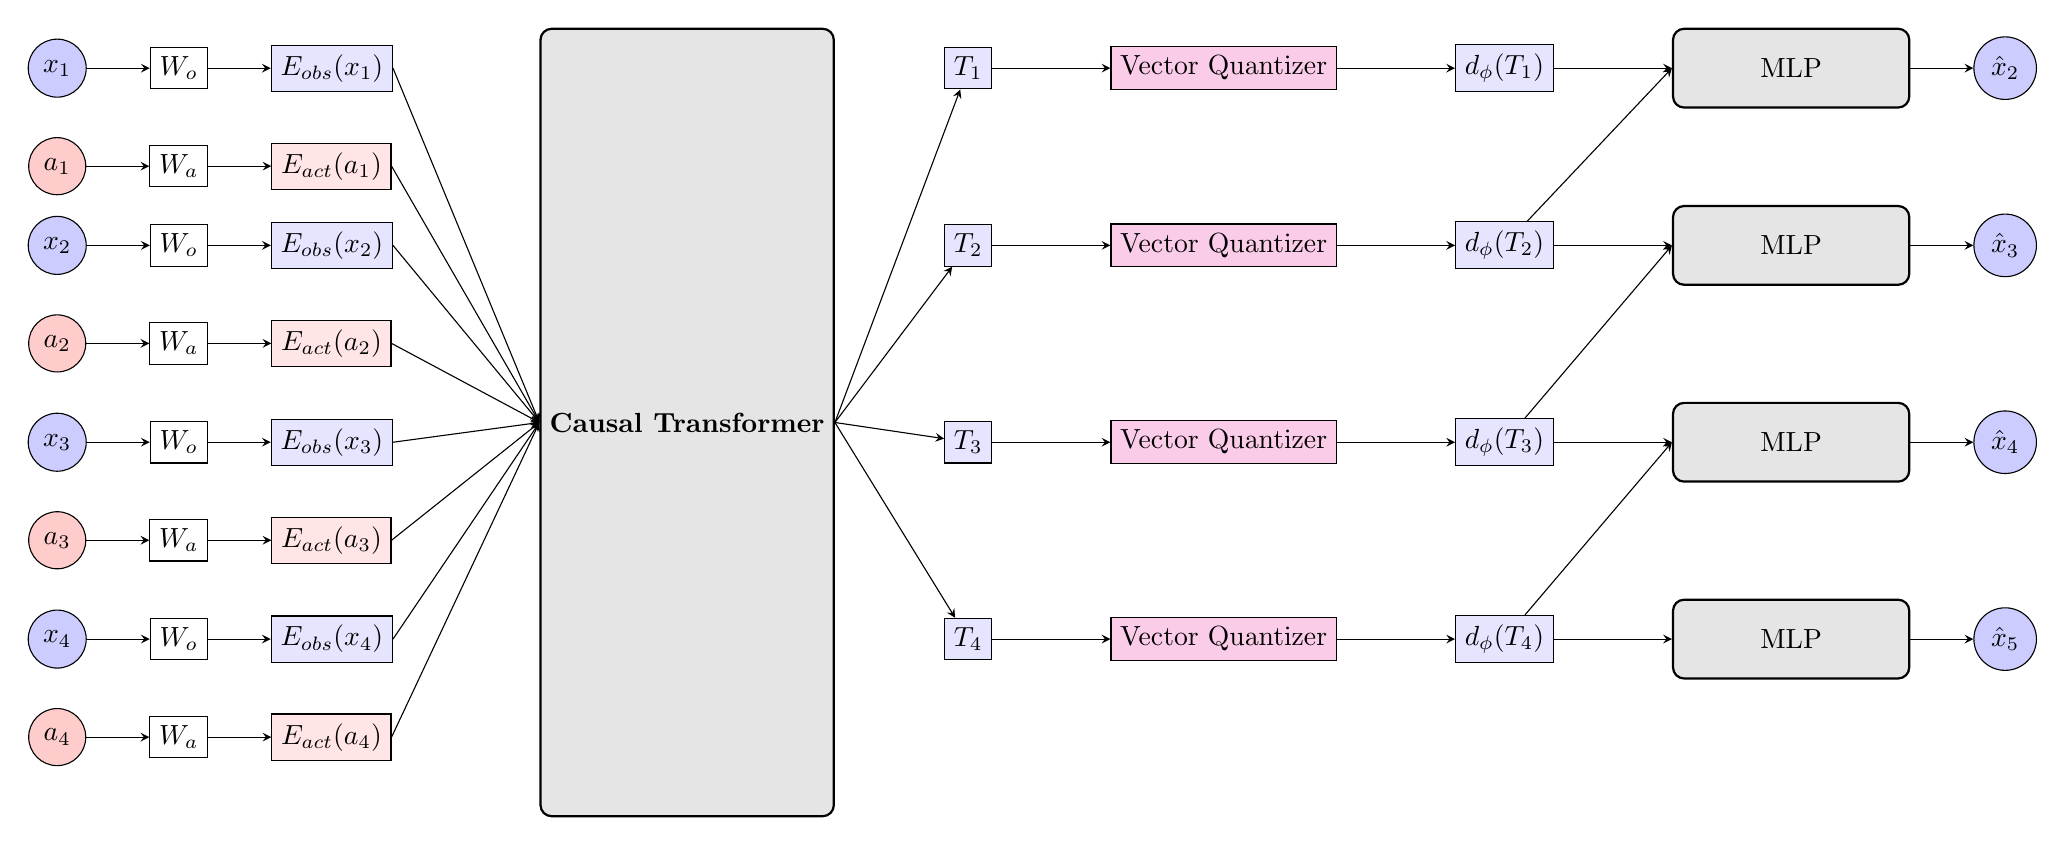
\begin{tikzpicture}[node distance=1.8cm,>=stealth]
      % Nodes for observations and actions at time 1
      \node[draw, circle, fill=blue!20] (obs1) {$x_1$};
      \node[draw, circle, fill=red!20, below=0.5cm of obs1] (act1) {$a_1$};
      \node[draw, right=0.8cm of obs1] (w0) {$W_o$};
      \node[draw, right=0.8cm of act1] (wa) {$W_a$};
      \node[draw, rectangle, fill=blue!10, right=0.8cm of w0] (eobs1) {$E_{obs}(x_1)$};
      \node[draw, rectangle, fill=red!10, right=0.8cm of wa] (eact1) {$E_{act}(a_1)$};
      
      % Transformer block
      \node[draw, thick, fill=gray!20, rounded corners, minimum width=3cm, minimum height=10cm] (transf) at (8,-4.5){\textbf{Causal Transformer}};
      
      % Vector quantizer
      \node[draw, rectangle, fill=blue!10, right=7 cm of eobs1] (t1) {$T_1$};
      \node[draw, fill=magenta!20, right=1.5cm of t1] (vq) {Vector Quantizer};
      \node[draw, rectangle, fill=blue!10, right=1.5cm of vq] (dq1) {$d_{\phi}(T_1)$};
      
      % Prediction MLP
      \node[draw, thick, fill=gray!20, rounded corners, minimum width=3cm, minimum height=1cm, right=1.5cm of dq1] (mlp1) {MLP};
      \node[draw, circle, fill=blue!20, right=0.8cm of mlp1] (xhat) {$\hat{x}_2$};
      
      % Connections for time 1
      \draw[->] (obs1) -- (w0);
      \draw[->] (act1) -- (wa);
      \draw[->] (w0) -- (eobs1);
      \draw[->] (wa) -- (eact1);
      \draw[->] (eobs1.east) -- (transf.west);
      \draw[->] (eact1.east) -- (transf.west);
      \draw[->] (transf.east) -- (t1);
      \draw[->] (t1) -- (vq);
      \draw[->] (vq) -- (dq1);
      \draw[->] (dq1) -- (mlp1);
      \draw[->] (mlp1) -- (xhat);
      
      % Additional time steps
      \foreach \i in {2,3,4} {
          \node[draw, circle, fill=blue!20, below=(\i-1)*2.5cm-1cm of obs1] (obs\i) {$x_\i$};
          \node[draw, circle, fill=red!20, below=0.5cm of obs\i] (act\i) {$a_\i$};
          \node[draw, right=0.8cm of obs\i] (w0\i) {$W_o$};
          \node[draw, right=0.8cm of act\i] (wa\i) {$W_a$};
          \node[draw, rectangle, fill=blue!10, right=0.8cm of w0\i] (eobs\i) {$E_{obs}(x_\i)$};
          \node[draw, rectangle, fill=red!10, right=0.8cm of wa\i] (eact\i) {$E_{act}(a_\i)$};
          %\node[draw, thick, fill=gray!20, rounded corners, minimum width=3cm, minimum height=2cm, right=1.5cm of eobs\i] (transf\i) {\textbf{Causal Transformer}};
          \node[draw, rectangle, fill=blue!10, right=7 cm of eobs\i] (t\i) {$T_\i$};
          \node[draw, fill=magenta!20, right=1.5cm of t\i] (vq\i) {Vector Quantizer};
          \node[draw, rectangle, fill=blue!10, right=1.5cm of vq\i] (dq\i) {$d_{\phi}(T_\i)$};
          \node[draw, thick, fill=gray!20, rounded corners, minimum width=3cm, minimum height=1cm, right=1.5cm of dq\i] (mlp\i) {MLP};
          \tikzmath{\j = \i+1;}

          
          % Connections for time \i
          \draw[->] (obs\i) -- (w0\i);
          \draw[->] (act\i) -- (wa\i);
          \draw[->] (w0\i) -- (eobs\i);
          \draw[->] (wa\i) -- (eact\i);
          \draw[->] (eobs\i.east) -- (transf.west);
          \draw[->] (eact\i.east) -- (transf.west);
          \draw[->] (transf.east) -- (t\i);
          \draw[->] (t\i) -- (vq\i);
          \draw[->] (vq\i) -- (dq\i);
          \draw[->] (dq\i) -- (mlp\i);
          
          
          % New arrow from d_phi(T_\i) to the MLP of the previous step
          
      }
      \draw[->] (dq2) -- (mlp1.west);
      \draw[->] (dq3) -- (mlp2.west);
      \draw[->] (dq4) -- (mlp3.west);
      
      \node[draw, circle, fill=blue!20, right=0.8cm of mlp2] (xhat2) {$\hat{x}_{3}$};
      \node[draw, circle, fill=blue!20, right=0.8cm of mlp3] (xhat3) {$\hat{x}_{4}$};
      \node[draw, circle, fill=blue!20, right=0.8cm of mlp4] (xhat4) {$\hat{x}_{5}$};
      \draw[->] (mlp2) -- (xhat2);
      \draw[->] (mlp3) -- (xhat3);
      \draw[->] (mlp4) -- (xhat4);
          
    \end{tikzpicture}}
\end{figure}

\end{document}
